\documentclass[10pt,aspectratio=43,mathserif]{beamer}
\usetheme{Boadilla} %主题

\usepackage[UTF8]{ctex} %中文化

\usepackage{graphicx} %导入图片
\graphicspath{{./images/}}

\usepackage{amsmath,bm,amsfonts,amssymb} %数学公式、符号等

\usepackage{tikz} %画图
\usetikzlibrary{calc,arrows,decorations.pathmorphing,intersections}
\tikzset{
    level/.style={black,thick},
    sublevel/.style={blue,densely dashed},
    ionization/.style={black,dashed},
	myarrow/.style={<->,decorate, draw=red,line width=0.4mm},
	myoutarrow/.style={|<->|,decorate, draw=red,line width=0.4mm},
	myline/.style={decorate, draw=red,line width=0.4mm},
    transition/.style={red,->,>=stealth',shorten >=1pt},
    radiative/.style={transition,decorate,decoration={snake,amplitude=1.5}},
    indirectradiative/.style={radiative,densely dashed},
    nonradiative/.style={transition,dashed}
}

\author{dc Lin}
\date{2018.9.1}

\begin{document}

\begin{frame}
\centering \LARGE
第七章、金属和半导体的接触
\end{frame}

\begin{frame}{7.1 金属半导体接触及其能级图--功函数和亲合能}
\begin{columns}
\begin{column}{0.5\textwidth}
\begin{block}{功函数(work function)}<1->
\small 用$E_0$表示真空中静止的电子能量,$(E_F)_m$是金属的费米能级,则$E_0-(E_F)_m$定义为金属的\textcolor<1->{red}{功函数},用$W_m$表示,它表示一个起始能量为费米能级的电子,从金属内部逸出到真空需要的最小能量,$W_m$越大,电子越不容易离开金属。
\end{block}
\end{column}

\begin{column}{0.5\textwidth}
\centerline{
%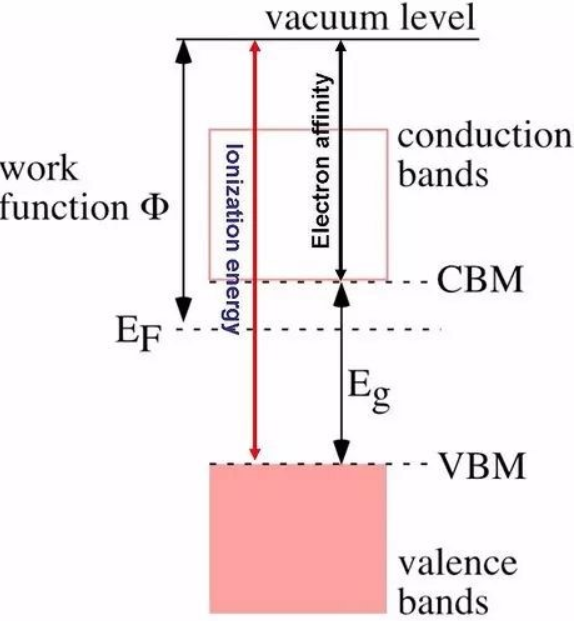
\includegraphics[width=0.7\textwidth]{work_function1.png}}
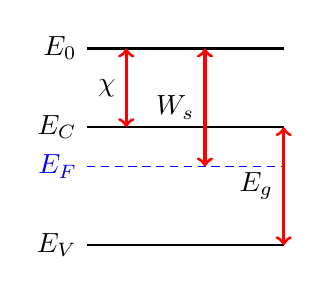
\begin{tikzpicture}[
	scale=0.5,
    font=\sffamily
]
%绘制能级
\draw[level] (0,9)node[left]{$E_0$}--(5,9); %E0
\draw[level] (0,7)node[left]{$E_C$}--(5,7); %EC
\draw[sublevel] (0,6)node[left]{$E_F$}--(5,6); %EF
\draw[level] (0,4)node[left]{$E_V$}--(5,4); %EV
%绘制标注线
\draw<2->[myarrow] (1,9)--(1,7)node[left, midway]{$\chi$};
\draw<1->[myarrow](3,9)--(3,6)node[left, midway]{$W_s$};
\draw[myarrow] (5,7)--(5,4)node[left, midway]{$E_g$};
\end{tikzpicture}
}
\end{column}
\end{columns}

\begin{block}{亲合能(Affinity energy)}<2->
\small 半导体的功函数:$W_s=E_0-(E_F)_s$,并把电子从导带最小能级跃迁到真空能级的最小能量称为\textcolor<2->{red}{亲合能},定义为:$\chi = E_0 - E_c$,所以$W_s=\chi+\left[E_c-(E_F)_s\right]$
\end{block}

\onslide<3->{参见材料功函数:铯(Cs, $1.93eV$, 金属最低), 铂(Pt, $5.36eV$, 金属最高), 硅(Si, $\chi=4.05eV$, 常温下,n型掺杂$N_D=10^{14}/cm^3$时,$W_s=4.37eV$, $N_D=10^{15}/cm^3$时,$W_s=4.31eV$, $N_D=10^{16}/cm^3$时,$W_s=4.25eV$)}
\end{frame}

\begin{frame}{接触电势差}

\begin{tabular}{ll}
%接触前
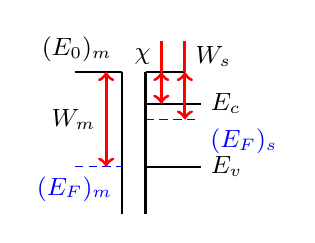
\begin{tikzpicture}[scale=0.2,font=\sffamily]
\draw[level] (0,9)--(3,9)node[above left]{\small$(E_0)_m$};
\draw[sublevel] (0,3)--(3,3)node[below left]{\small$(E_F)_m$};
\draw[level] (3,9)--(3,0);
\draw[myarrow] (2,9)--(2,3)node[left, midway]{\small$W_m$};

\draw[level] (4.5,9)--(7,9);
\draw[level] (4.5,7)--(8,7)node[right]{\small$E_c$};
\draw[sublevel] (4.5,6)--(8,6)node[below right]{\small$(E_F)_s$};
\draw[level] (4.5,3)--(8,3)node[right]{\small$E_v$};
\draw[level] (4.5,9)--(4.5,0);

\draw[myarrow] (5.5,9)--(5.5,7);
\draw[myline](5.5,9)--node[left, midway]{\small$\chi$}(5.5,11);

\draw[myarrow] (7,9)--(7,6);
\draw[myline](7,9)--node[right, midway]{\small$W_s$}(7,11);

\end{tikzpicture} 

%间隙很大
&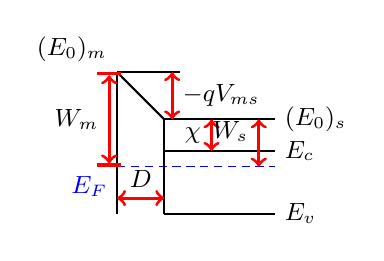
\begin{tikzpicture}[scale=0.2,font=\sffamily]
\draw[level] (0,9)node[above left]{\small$(E_0)_m$}--(4,9);
\draw[sublevel] (0,3)node[below left]{\small$E_F$}--(10,3);
\draw[level] (3,6)--(10,6)node[right]{\small$(E_0)_s$};
\draw[level] (3,4)--(10,4)node[right]{\small$E_c$};
\draw[level] (3,0)--(10,0)node[right]{\small$E_v$};
\draw[level](0,0)--(0,9);
\draw[level](3,0)--(3,6);
\draw[level](0,9)--(3,6);
\draw[myarrow] (0,1)--(3,1)node[above, midway]{\small$D$};
\draw[myoutarrow] (-0.5,9)--(-0.5,3)node[left, midway]{\small$W_m$};
\draw[myarrow] (3.5,9)--(3.5,6)node[right,midway]{\small$-qV_{ms}$};
\draw[myarrow] (6,6)--(6,4)node[left, midway]{\small$\chi$};
\draw[myarrow] (9,6)--(9,3)node[left, pos=0.25]{\small$W_s$};
\end{tikzpicture} \\

(a) 接触前 &(b) 间隙很大 \\

%紧密接触
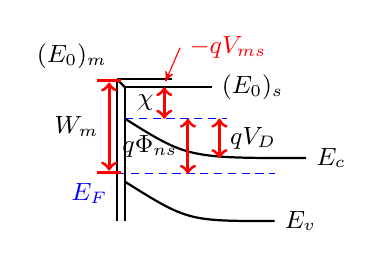
\begin{tikzpicture}[scale=0.2,font=\sffamily]
\draw[level](0,9)node[above left]{\small$(E_0)_m$}--(3.5,9);
\draw[sublevel] (0,3)node[below left]{\small$E_F$}--(10,3);
\draw[level](0,9)--(0,0);
\draw[level](0.5,8.5)--(6,8.5)node[right]{\small$(E_0)_s$};
\draw[level](0.5,8.5)--(0.5,0);
\draw[level](0.5,8.5)--(0,9);
\draw[level](0.5,6.5)..controls(4.5,4)..(12,4)node[right]{\small$E_c$};
\draw[level](0.5,2.5)..controls(4.5,0)..(10,0)node[right]{\small$E_v$};
\draw[sublevel] (0.5,6.5)--(7,6.5);
\draw[myoutarrow] (-0.5,9)--(-0.5,3)node[left, midway]{\small$W_m$};
\draw[myarrow] (6.5,6.5)--(6.5,4)node[right, midway]{\small$qV_D$};
\draw[myarrow] (4.5,6.5)--(4.5,3)node[left, midway]{\small$q\Phi_{ns}$};
\draw[myarrow] (3,8.5)--(3,6.5)node[left, midway]{\small$\chi$};
\draw[transition] (4,11)node[right]{\small$-qV_{ms}$}--(3,8.7);
\end{tikzpicture}

&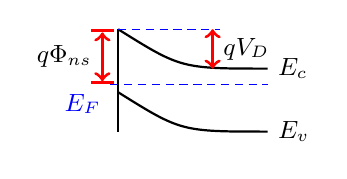
\begin{tikzpicture}[scale=0.2,font=\sffamily]
\draw[sublevel] (0,3)node[below left]{\small$E_F$}--(10,3);
\draw[level](0.5,6.5)--(0.5,0);
\draw[level](0.5,6.5)..controls(4.5,4)..(10,4)node[right]{\small$E_c$};
\draw[level](0.5,2.5)..controls(4.5,0)..(10,0)node[right]{\small$E_v$};
\draw[sublevel] (0.5,6.5)--(7,6.5);
\draw[myarrow] (6.5,6.5)--(6.5,4)node[right, midway]{\small$qV_D$};
\draw[myoutarrow] (-0.5,6.5)--(-0.5,3)node[left, midway]{\small$q\Phi_{ns}$};
\end{tikzpicture}  \\

(c) 紧密接触 &(d) 忽略间隙 
\end{tabular}

这里是假设半导体是n型,$W_m > W_s$, $V_{ms}$是\textcolor{red}{接触电势差},$V_D$是半导体的空间电荷区内电场电压,$q\Phi_{ns}$是金属的势垒高度,$qV_D$是半导体势垒的高度。

\end{frame}

\begin{frame}{阻挡层和反阻挡层}

\begin{tabular}{ll}
%n型半导体和金属接触:阻挡层
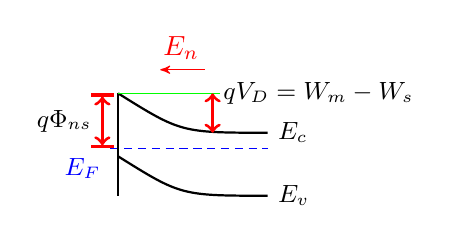
\begin{tikzpicture}[scale=0.2,font=\sffamily]
\draw[sublevel] (0,3)node[below left]{\small$E_F$}--(10,3);
\draw[level](0.5,6.5)--(0.5,0);
\draw[level](0.5,6.5)..controls(4.5,4)..(10,4)node[right]{\small$E_c$};
\draw[level](0.5,2.5)..controls(4.5,0)..(10,0)node[right]{\small$E_v$};
\draw[green] (0.5,6.5)--(7,6.5);
\draw[myarrow] (6.5,6.5)--(6.5,4)node[right, pos=0]{\small$qV_D=W_m-W_s$};
\draw[myoutarrow] (-0.5,6.5)--(-0.5,3)node[left, midway]{\small$q\Phi_{ns}$};
\draw[transition](6,8)--(3,8)node[above,midway]{$E_n$};
\end{tikzpicture} 

%n型半导体和金属接触:反阻挡层
&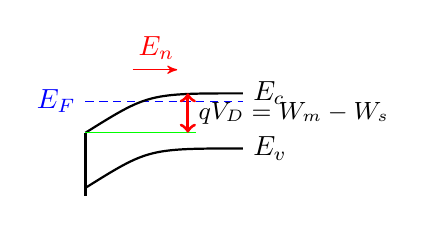
\begin{tikzpicture}[scale=0.2,font=\sffamily]
\draw[level](0,0)--(0,4);
\draw[sublevel](0,6)node[left]{$E_F$}--(10,6);
\draw[level](0,4)..controls(4,6.5)..(10,6.5)node[right]{$E_c$};
\draw[level](0,0.5)..controls(4,3)..(10,3)node[right]{$E_v$};
\draw[green](0,4)--(7,4);
\draw[myarrow](6.5,6.5)--(6.5,4)node[right, midway]{\small$qV_D=W_m-W_s$};
\draw[transition](3,8)--(6,8)node[above,midway]{$E_n$};
\end{tikzpicture} \\

(a)n型阻挡层($W_m > W_s$) &(b)n型反阻挡层($W_m < W_s$) \\

%p型半导体和金属接触:阻挡层
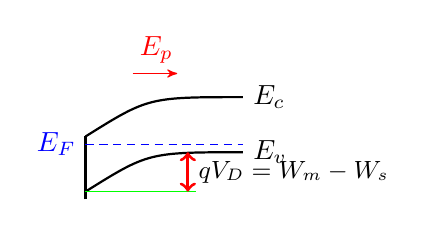
\begin{tikzpicture}[scale=0.2,font=\sffamily]
\draw[level](0,0)--(0,4);
\draw[sublevel](0,3.5)node[left]{$E_F$}--(10,3.5);
\draw[level](0,4)..controls(4,6.5)..(10,6.5)node[right]{$E_c$};
\draw[level](0,0.5)..controls(4,3)..(10,3)node[right]{$E_v$};
\draw[green](0,0.5)--(7,0.5);
\draw[myarrow](6.5,0.5)--(6.5,3)node[right, midway]{\small$qV_D=W_m-W_s$};
\draw[transition](3,8)--(6,8)node[above,midway]{$E_p$};
\end{tikzpicture}

%p型半导体和金属接触:反阻挡层
&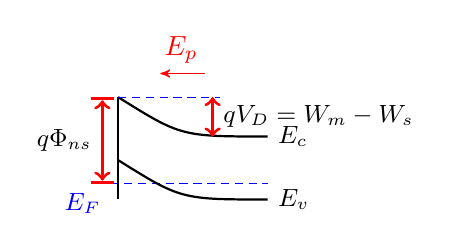
\begin{tikzpicture}[scale=0.2,font=\sffamily]
\draw[sublevel] (0,1)node[below left]{\small$E_F$}--(10,1);
\draw[level](0.5,6.5)--(0.5,0);
\draw[level](0.5,6.5)..controls(4.5,4)..(10,4)node[right]{\small$E_c$};
\draw[level](0.5,2.5)..controls(4.5,0)..(10,0)node[right]{\small$E_v$};
\draw[sublevel] (0.5,6.5)--(7,6.5);
\draw[myarrow] (6.5,6.5)--(6.5,4)node[right, midway]{\small$qV_D=W_m-W_s$};
\draw[myoutarrow] (-0.5,6.5)--(-0.5,1)node[left, midway]{\small$q\Phi_{ns}$};
\draw[transition](6,8)--(3,8)node[above,midway]{$E_p$};
\end{tikzpicture}  \\

(c)p型阻挡层($W_m < W_s$) &(d)p型反阻挡层($W_m > W_s$) 
\end{tabular}

\end{frame}

\begin{frame}{7.2 金属半导体接触整流}

\begin{tabular}{ll}

\begin{tikzpicture}[scale=0.16]
\draw[level](0,4.5)rectangle(2.5,0.5);
\draw[level](6,4.5)rectangle(10 ,0.5);
\draw[level](2.5,4.5) rectangle (6,0.5);
\foreach \x in {3,...,5}
	\foreach \y in {1,...,4}
		{\draw[level](\x,\y)--(\x+0.5,\y);
		 \draw[level](\x+0.25,\y+0.25)--(\x+0.25,\y-0.25);
		}
\node at(0,6){金属};
\node at(8,6){半导体};

\draw[level](2.5, -1)--(2.5, -7);
\draw[level](2.5, -1)..controls(5, -6)..(10, -6)node[below right]{$E_c$};
\draw[blue,dashed](2.5,-1)--(8,-1);
\draw[myarrow](6,-1)--(6,-6)node[right,midway]{\small $qV_D=-q(V_s)_0$};
\draw[transition](7, 8)node[right]{$E_{in}$}--(1,8);
\end{tikzpicture}

&\begin{tikzpicture}[scale=0.16]
\draw[level](0,4.5)rectangle(2.5,0.5);
\draw[level](6,4.5)rectangle(10 ,0.5);
\draw[level](2.5,4.5) rectangle (6,0.5);
\foreach \x in {3,...,5}
	\foreach \y in {1,...,4}
		{\draw[level](\x,\y)--(\x+0.5,\y);
		 \draw[level](\x+0.25,\y+0.25)--(\x+0.25,\y-0.25);
		}
\node at(0,6){金属};
\node at(8,6){半导体};
\node at(1,3){\textcircled{+}};

\draw[level](2.5, -1)--(2.5, -5);
\draw[level](2.5, -1)..controls(5, -4)..(10, -4)node[below right]{$E_c$};
\draw[blue,dashed](2.5,-1)--(8,-1);
\draw[myarrow](6,-1)--(6,-4)node[right,midway]{\small $-q[(V_s)_0-V]$};
\draw[transition](7, 8)node[right]{$E_{in}$}--(1,8);
\draw[transition](1, 10)node[left]{$E_{out}$}--(7,10);
\end{tikzpicture} \\

(a)$V=0$ &(b)$V>0$ \\

\begin{tikzpicture}[scale=0.16]
\draw[level](0,4.5)rectangle(2.5,0.5);
\draw[level](6,4.5)rectangle(10 ,0.5);
\draw[level](2.5,4.5) rectangle (6,0.5);
\foreach \x in {3,...,5}
	\foreach \y in {1,...,4}
		{\draw[level](\x,\y)--(\x+0.5,\y);
		 \draw[level](\x+0.25,\y+0.25)--(\x+0.25,\y-0.25);
		}
\node at(0,6){金属};
\node at(8,6){半导体};
\node at(7,3){\textcircled{+}};

\draw[level](2.5, -1)--(2.5, -9);
\draw[level](2.5, -1)..controls(5, -8)..(10, -8)node[below right]{$E_c$};
\draw[blue,dashed](2.5,-1)--(8,-1);
\draw[myarrow](6,-1)--(6,-8)node[right,midway]{\small $-q[(V_s)_0+V]$};
\draw[transition](7, 8)node[right]{$E_{in}$}--(1,8);
\draw[transition](7, 10)node[right]{$E_{out}$}--(1,10);
\end{tikzpicture} 

&\begin{tikzpicture}[scale=0.3]
\draw[transition](-5,0)--(5,0)node[right]{$V$};
\draw[transition]( 0,-2)--(0,10)node[left]{$I$};
\draw[level](0,0)..controls(1,0)..(2, 9);
\draw[level](0,0)..controls(-2,-1)..(-5, -1);
\end{tikzpicture}  \\

(c)$V<0$  &(d)金属半导体接触伏安特性曲线
\end{tabular}

\end{frame}

\begin{frame}{7.3 肖特基势垒二极管}

\begin{columns}

\begin{column}{0.6\textwidth}
\begin{block}{肖特基势垒二极管}
肖特基二极管是利用金属-半导体接面作为肖特基势垒,以产生\textcolor{red}{整流}的效果,和一般二极管中由半导体-半导体接面产生的P-N结不同。肖特基势垒的特性(多子扩散)使得肖特基二极管的\textcolor{red}{导通电压降较低}(pn结硅管是$0.7V$,肖特基管一般$0.3V$),而且可以\textcolor{blue}{提高切换的速度}。
\end{block}
\end{column}

\begin{column}{0.4\textwidth}
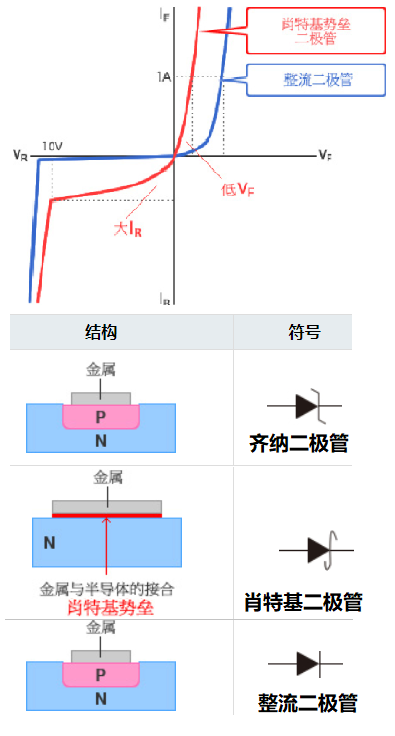
\includegraphics[width=0.7\textwidth]{二极管.png}
\end{column}

\end{columns}
\end{frame}

\begin{frame}{7.4 欧姆接触 Ohmic contact}
	\begin{columns}
		\begin{column}{0.6\textwidth}
			\small
			\begin{block}{肖特基接触}
				像上节所说,在金属和半导体接触时,出现阻挡层,导致出现整流(rectifying)的状况(也就是单向导通),\textcolor{red}{半导体体内的载流子流向体表会有阻碍,这就是肖特基接触}。
			\end{block}
			
			\begin{block}{欧姆接触}
				在金属和半导体接触时,没有对体内载流子流向体表产生阻碍,而是\textcolor{blue}{正常的具有线性的电流-电压特性曲线,这种接触就是欧姆接触}。
				
				要形成欧姆接触,可以采用\textcolor{red}{反阻挡层}(也就是$W_m>W_s$),但是由于半导体的表面态密度很高,所以提高金属的功函数可行性不高,实际生产是\textcolor{green}{采用隧道原理}来实现。在第六章中知道,可以\textcolor{red}{通过重掺杂的pn结来实现隧道电流}。
			\end{block}
		\end{column}
		\begin{column}{0.4\textwidth}
			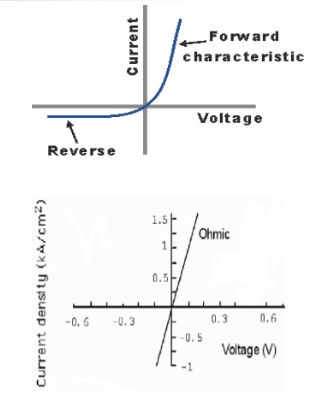
\includegraphics[width=0.9\textwidth]{ohmic_contacts.png}
		\end{column}
	\end{columns}
\end{frame}
\end{document}